% Options for packages loaded elsewhere
\PassOptionsToPackage{unicode}{hyperref}
\PassOptionsToPackage{hyphens}{url}
\PassOptionsToPackage{dvipsnames,svgnames,x11names}{xcolor}
%
\documentclass[
  letterpaper,
  DIV=11,
  numbers=noendperiod]{scrartcl}

\usepackage{amsmath,amssymb}
\usepackage{lmodern}
\usepackage{iftex}
\ifPDFTeX
  \usepackage[T1]{fontenc}
  \usepackage[utf8]{inputenc}
  \usepackage{textcomp} % provide euro and other symbols
\else % if luatex or xetex
  \usepackage{unicode-math}
  \defaultfontfeatures{Scale=MatchLowercase}
  \defaultfontfeatures[\rmfamily]{Ligatures=TeX,Scale=1}
\fi
% Use upquote if available, for straight quotes in verbatim environments
\IfFileExists{upquote.sty}{\usepackage{upquote}}{}
\IfFileExists{microtype.sty}{% use microtype if available
  \usepackage[]{microtype}
  \UseMicrotypeSet[protrusion]{basicmath} % disable protrusion for tt fonts
}{}
\makeatletter
\@ifundefined{KOMAClassName}{% if non-KOMA class
  \IfFileExists{parskip.sty}{%
    \usepackage{parskip}
  }{% else
    \setlength{\parindent}{0pt}
    \setlength{\parskip}{6pt plus 2pt minus 1pt}}
}{% if KOMA class
  \KOMAoptions{parskip=half}}
\makeatother
\usepackage{xcolor}
\setlength{\emergencystretch}{3em} % prevent overfull lines
\setcounter{secnumdepth}{-\maxdimen} % remove section numbering
% Make \paragraph and \subparagraph free-standing
\ifx\paragraph\undefined\else
  \let\oldparagraph\paragraph
  \renewcommand{\paragraph}[1]{\oldparagraph{#1}\mbox{}}
\fi
\ifx\subparagraph\undefined\else
  \let\oldsubparagraph\subparagraph
  \renewcommand{\subparagraph}[1]{\oldsubparagraph{#1}\mbox{}}
\fi

\usepackage{color}
\usepackage{fancyvrb}
\newcommand{\VerbBar}{|}
\newcommand{\VERB}{\Verb[commandchars=\\\{\}]}
\DefineVerbatimEnvironment{Highlighting}{Verbatim}{commandchars=\\\{\}}
% Add ',fontsize=\small' for more characters per line
\usepackage{framed}
\definecolor{shadecolor}{RGB}{241,243,245}
\newenvironment{Shaded}{\begin{snugshade}}{\end{snugshade}}
\newcommand{\AlertTok}[1]{\textcolor[rgb]{0.68,0.00,0.00}{#1}}
\newcommand{\AnnotationTok}[1]{\textcolor[rgb]{0.37,0.37,0.37}{#1}}
\newcommand{\AttributeTok}[1]{\textcolor[rgb]{0.40,0.45,0.13}{#1}}
\newcommand{\BaseNTok}[1]{\textcolor[rgb]{0.68,0.00,0.00}{#1}}
\newcommand{\BuiltInTok}[1]{\textcolor[rgb]{0.00,0.23,0.31}{#1}}
\newcommand{\CharTok}[1]{\textcolor[rgb]{0.13,0.47,0.30}{#1}}
\newcommand{\CommentTok}[1]{\textcolor[rgb]{0.37,0.37,0.37}{#1}}
\newcommand{\CommentVarTok}[1]{\textcolor[rgb]{0.37,0.37,0.37}{\textit{#1}}}
\newcommand{\ConstantTok}[1]{\textcolor[rgb]{0.56,0.35,0.01}{#1}}
\newcommand{\ControlFlowTok}[1]{\textcolor[rgb]{0.00,0.23,0.31}{#1}}
\newcommand{\DataTypeTok}[1]{\textcolor[rgb]{0.68,0.00,0.00}{#1}}
\newcommand{\DecValTok}[1]{\textcolor[rgb]{0.68,0.00,0.00}{#1}}
\newcommand{\DocumentationTok}[1]{\textcolor[rgb]{0.37,0.37,0.37}{\textit{#1}}}
\newcommand{\ErrorTok}[1]{\textcolor[rgb]{0.68,0.00,0.00}{#1}}
\newcommand{\ExtensionTok}[1]{\textcolor[rgb]{0.00,0.23,0.31}{#1}}
\newcommand{\FloatTok}[1]{\textcolor[rgb]{0.68,0.00,0.00}{#1}}
\newcommand{\FunctionTok}[1]{\textcolor[rgb]{0.28,0.35,0.67}{#1}}
\newcommand{\ImportTok}[1]{\textcolor[rgb]{0.00,0.46,0.62}{#1}}
\newcommand{\InformationTok}[1]{\textcolor[rgb]{0.37,0.37,0.37}{#1}}
\newcommand{\KeywordTok}[1]{\textcolor[rgb]{0.00,0.23,0.31}{#1}}
\newcommand{\NormalTok}[1]{\textcolor[rgb]{0.00,0.23,0.31}{#1}}
\newcommand{\OperatorTok}[1]{\textcolor[rgb]{0.37,0.37,0.37}{#1}}
\newcommand{\OtherTok}[1]{\textcolor[rgb]{0.00,0.23,0.31}{#1}}
\newcommand{\PreprocessorTok}[1]{\textcolor[rgb]{0.68,0.00,0.00}{#1}}
\newcommand{\RegionMarkerTok}[1]{\textcolor[rgb]{0.00,0.23,0.31}{#1}}
\newcommand{\SpecialCharTok}[1]{\textcolor[rgb]{0.37,0.37,0.37}{#1}}
\newcommand{\SpecialStringTok}[1]{\textcolor[rgb]{0.13,0.47,0.30}{#1}}
\newcommand{\StringTok}[1]{\textcolor[rgb]{0.13,0.47,0.30}{#1}}
\newcommand{\VariableTok}[1]{\textcolor[rgb]{0.07,0.07,0.07}{#1}}
\newcommand{\VerbatimStringTok}[1]{\textcolor[rgb]{0.13,0.47,0.30}{#1}}
\newcommand{\WarningTok}[1]{\textcolor[rgb]{0.37,0.37,0.37}{\textit{#1}}}

\providecommand{\tightlist}{%
  \setlength{\itemsep}{0pt}\setlength{\parskip}{0pt}}\usepackage{longtable,booktabs,array}
\usepackage{calc} % for calculating minipage widths
% Correct order of tables after \paragraph or \subparagraph
\usepackage{etoolbox}
\makeatletter
\patchcmd\longtable{\par}{\if@noskipsec\mbox{}\fi\par}{}{}
\makeatother
% Allow footnotes in longtable head/foot
\IfFileExists{footnotehyper.sty}{\usepackage{footnotehyper}}{\usepackage{footnote}}
\makesavenoteenv{longtable}
\usepackage{graphicx}
\makeatletter
\def\maxwidth{\ifdim\Gin@nat@width>\linewidth\linewidth\else\Gin@nat@width\fi}
\def\maxheight{\ifdim\Gin@nat@height>\textheight\textheight\else\Gin@nat@height\fi}
\makeatother
% Scale images if necessary, so that they will not overflow the page
% margins by default, and it is still possible to overwrite the defaults
% using explicit options in \includegraphics[width, height, ...]{}
\setkeys{Gin}{width=\maxwidth,height=\maxheight,keepaspectratio}
% Set default figure placement to htbp
\makeatletter
\def\fps@figure{htbp}
\makeatother

\KOMAoption{captions}{tableheading}
\makeatletter
\makeatother
\makeatletter
\makeatother
\makeatletter
\@ifpackageloaded{caption}{}{\usepackage{caption}}
\AtBeginDocument{%
\ifdefined\contentsname
  \renewcommand*\contentsname{Table of contents}
\else
  \newcommand\contentsname{Table of contents}
\fi
\ifdefined\listfigurename
  \renewcommand*\listfigurename{List of Figures}
\else
  \newcommand\listfigurename{List of Figures}
\fi
\ifdefined\listtablename
  \renewcommand*\listtablename{List of Tables}
\else
  \newcommand\listtablename{List of Tables}
\fi
\ifdefined\figurename
  \renewcommand*\figurename{Figure}
\else
  \newcommand\figurename{Figure}
\fi
\ifdefined\tablename
  \renewcommand*\tablename{Table}
\else
  \newcommand\tablename{Table}
\fi
}
\@ifpackageloaded{float}{}{\usepackage{float}}
\floatstyle{ruled}
\@ifundefined{c@chapter}{\newfloat{codelisting}{h}{lop}}{\newfloat{codelisting}{h}{lop}[chapter]}
\floatname{codelisting}{Listing}
\newcommand*\listoflistings{\listof{codelisting}{List of Listings}}
\makeatother
\makeatletter
\@ifpackageloaded{caption}{}{\usepackage{caption}}
\@ifpackageloaded{subcaption}{}{\usepackage{subcaption}}
\makeatother
\makeatletter
\@ifpackageloaded{tcolorbox}{}{\usepackage[many]{tcolorbox}}
\makeatother
\makeatletter
\@ifundefined{shadecolor}{\definecolor{shadecolor}{rgb}{.97, .97, .97}}
\makeatother
\makeatletter
\makeatother
\ifLuaTeX
  \usepackage{selnolig}  % disable illegal ligatures
\fi
\IfFileExists{bookmark.sty}{\usepackage{bookmark}}{\usepackage{hyperref}}
\IfFileExists{xurl.sty}{\usepackage{xurl}}{} % add URL line breaks if available
\urlstyle{same} % disable monospaced font for URLs
\hypersetup{
  pdftitle={CV\_communities2},
  pdfauthor={Suzana Blake},
  colorlinks=true,
  linkcolor={blue},
  filecolor={Maroon},
  citecolor={Blue},
  urlcolor={Blue},
  pdfcreator={LaTeX via pandoc}}

\title{CV\_communities2}
\author{Suzana Blake}
\date{}

\begin{document}
\maketitle
\ifdefined\Shaded\renewenvironment{Shaded}{\begin{tcolorbox}[enhanced, borderline west={3pt}{0pt}{shadecolor}, boxrule=0pt, breakable, interior hidden, frame hidden, sharp corners]}{\end{tcolorbox}}\fi

\textbf{Method Description:} Coefficient of Variation (CV):

The Coefficient\_of\_Variation is a measure of relative variability and
is calculated as the standard deviation divided by the mean, expressed
as a percentage. In the context of your analysis, a higher
Coefficient\_of\_Variation indicates greater relative variability in the
Total\_Val values over the years for a particular city.

So, the resulting DataFrame high\_variability\_cities gives you a list
of cities where the landed fish values have the highest year-to-year
variability based on the calculated coefficient of variation. Cities
with higher values in this DataFrame are those that experience more
significant fluctuations in the total landed fish values from one year
to the next.

A coefficient of variation (CV) value of 100.6 for a city indicates a
relatively high degree of variability in the context of your data. The
coefficient of variation is expressed as a percentage and is calculated
as the standard deviation divided by the mean, multiplied by 100.

Mathematically, CV is calculated using the formula:

\textbf{CV=(SDMean)×100CV=( MeanSD\hspace{0pt} )×100}

Here:

SD is the standard deviation of the variable of interest (e.g., total
landed fish values for a city). Mean is the mean (average) of the
variable. A CV value greater than 100\% implies that the standard
deviation is larger than the mean, indicating substantial relative
variability. It suggests that the data points (total landed fish values)
are widely spread out from the mean, which could be due to fluctuations
or volatility in the values over time.

In practical terms, a CV value of 100.6 indicates that the variability
in the total landed fish values for that city is substantial, and the
mean may not be a reliable summary measure on its own. Analysts often
use the CV to assess the relative dispersion or stability of a variable,
and a higher CV suggests higher relative variability.

Note: When calculating the coefficient of variation (CV) for a city, the
mean (average) is computed based on the values available for that
specific city across the years where data is available. It doesn't
consider data from other cities or years.

What constitutes Low and High Variability?

\textbf{Low Variability:}

In many cases, a CV below 10\% is considered relatively low variability.
This implies that the standard deviation is small compared to the mean,
suggesting that the values are closely clustered around the average.

\textbf{Moderate Variability:}

A CV between 10\% and 30\% is often considered moderate variability. It
indicates a moderate level of dispersion around the mean.

\textbf{High Variability:}

A CV above 30\% is generally considered high variability. This suggests
that the values are more spread out, and there is a substantial degree
of fluctuation relative to the mean.

\textbf{Dataset-specific Considerations:}

The definition of low variability can vary depending on the nature of
the data and the specific industry or field. Some datasets inherently
have higher variability due to the nature of the measurements.

\textbf{This is what where we need to have a conversation about how we
will define high and low variability} because as you will see in the
analysis below most of the data points have variability that would be
considered by general standards to be moderate to high variability.

\#\#\textbf{Data organization}

Load Inflation Adjusted Data

Brief summary

\begin{Shaded}
\begin{Highlighting}[]
\CommentTok{\# Display a summary of the GI data}
\FunctionTok{summary}\NormalTok{(GI)}
\end{Highlighting}
\end{Shaded}

\begin{verbatim}
  landed_year   data_supplier_st    dealer_id         corporate_name    
 Min.   :1977   Length:475823      Length:475823      Length:475823     
 1st Qu.:1993   Class :character   Class :character   Class :character  
 Median :2002   Mode  :character   Mode  :character   Mode  :character  
 Mean   :2001                                                           
 3rd Qu.:2011                                                           
 Max.   :2020                                                           
                                                                        
 dealer_state       county_name        dealer_city          zipcode         
 Length:475823      Length:475823      Length:475823      Length:475823     
 Class :character   Class :character   Class :character   Class :character  
 Mode  :character   Mode  :character   Mode  :character   Mode  :character  
                                                                            
                                                                            
                                                                            
                                                                            
  species_itis    common_name           live_lbs             value         
 Min.   :  5414   Length:475823      Min.   :      -10   Min.   :    -190  
 1st Qu.:161092   Class :character   1st Qu.:       41   1st Qu.:      53  
 Median :168791   Mode  :character   Median :      322   Median :     401  
 Mean   :192794                      Mean   :    96661   Mean   :   66539  
 3rd Qu.:170335                      3rd Qu.:     3380   3rd Qu.:    4386  
 Max.   :775091                      Max.   :602540946   Max.   :78082845  
 NA's   :9                           NA's   :997         NA's   :20353     
 Inflation_index  Adjust_factor    Adjusted_Val     
 Min.   : 33.43   Min.   :1.000   Min.   :    -207  
 1st Qu.: 68.88   1st Qu.:1.159   1st Qu.:      74  
 Median : 81.03   Median :1.404   Median :     563  
 Mean   : 81.87   Mean   :1.482   Mean   :  103924  
 3rd Qu.: 98.16   3rd Qu.:1.652   3rd Qu.:    6195  
 Max.   :113.78   Max.   :3.404   Max.   :80520745  
                                  NA's   :20353     
\end{verbatim}

\begin{Shaded}
\begin{Highlighting}[]
\CommentTok{\# Create a plot using the GI data}
\FunctionTok{plot}\NormalTok{(GI}\SpecialCharTok{$}\NormalTok{landed\_year, GI}\SpecialCharTok{$}\NormalTok{Adjusted\_Val, }\AttributeTok{type =} \StringTok{"l"}\NormalTok{, }\AttributeTok{main =} \StringTok{"Adjusted Value Over Time"}\NormalTok{)}
\end{Highlighting}
\end{Shaded}

\begin{figure}[H]

{\centering 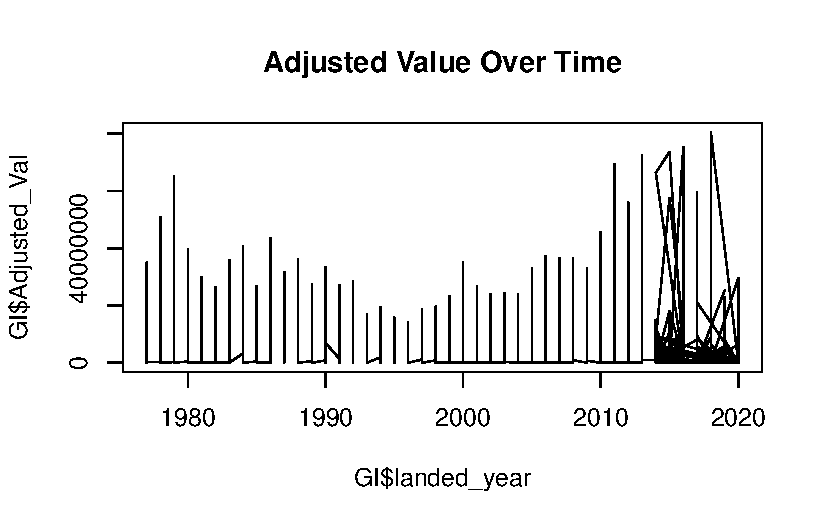
\includegraphics{CV_Communities2_files/figure-pdf/unnamed-chunk-2-1.pdf}

}

\end{figure}

\#\#\#Clean and group the Species names

\hypertarget{most-valuable-species}{%
\subsection{Most Valuable Species}\label{most-valuable-species}}

Identify the most Valuable Commercial Fish Species landed in the Gulf of
Mexico

\begin{Shaded}
\begin{Highlighting}[]
\CommentTok{\# Group by fish species and calculate the total adjusted value}
\NormalTok{most\_valuable }\OtherTok{\textless{}{-}}\NormalTok{ GI }\SpecialCharTok{\%\textgreater{}\%}
  \FunctionTok{group\_by}\NormalTok{(common\_name\_cleaned) }\SpecialCharTok{\%\textgreater{}\%}
  \FunctionTok{summarise}\NormalTok{(}\AttributeTok{total\_adjusted\_value =} \FunctionTok{sum}\NormalTok{(Adjusted\_Val, }\AttributeTok{na.rm =} \ConstantTok{TRUE}\NormalTok{)) }\SpecialCharTok{\%\textgreater{}\%}
  \FunctionTok{arrange}\NormalTok{(}\FunctionTok{desc}\NormalTok{(total\_adjusted\_value))}

\CommentTok{\# Print the table of fish species sorted by total adjusted value}
\FunctionTok{print}\NormalTok{(most\_valuable)}
\end{Highlighting}
\end{Shaded}

\begin{verbatim}
# A tibble: 824 x 2
   common_name_cleaned total_adjusted_value
   <chr>                              <dbl>
 1 Brown Shrimp                 17662967920
 2 White Shrimp                 12511132805
 3 Pink Shrimp                   2897587320
 4 OYSTER, EASTERN               2745493994
 5 MENHADENS                     2443102691
 6 Blue Crab                     1493188136
 7 Spiny Lobster                 1344745704
 8 Stone Crab                    1096418580
 9 Snapper                        949368835
10 Grouper                        883207380
# i 814 more rows
\end{verbatim}

\#\#Top 10 most valuable species

\begin{Shaded}
\begin{Highlighting}[]
\FunctionTok{library}\NormalTok{(dplyr)}

\NormalTok{Most\_Val }\OtherTok{\textless{}{-}} \FunctionTok{c}\NormalTok{(}\StringTok{"Brown Shrimp"}\NormalTok{,}\StringTok{"White Shrimp"}\NormalTok{,}\StringTok{"Pink Shrimp"}\NormalTok{, }\StringTok{"OYSTER, EASTERN"}\NormalTok{, }\StringTok{"Blue Crab"}\NormalTok{, }\StringTok{"Spiny Lobster"}\NormalTok{, }\StringTok{"Stone Crab"}\NormalTok{, }\StringTok{"Snapper"}\NormalTok{, }\StringTok{"Grouper"}\NormalTok{) }\CommentTok{\# excluded Menhadens}

\CommentTok{\# Create a new data frame with only the top 10 species}
\NormalTok{top\_10\_data }\OtherTok{\textless{}{-}}\NormalTok{ GI }\SpecialCharTok{\%\textgreater{}\%}
  \FunctionTok{filter}\NormalTok{(common\_name }\SpecialCharTok{\%in\%}\NormalTok{ Most\_Val) }\CommentTok{\# this has over 50,000 records which is much smaller than the original data file which has so many more species}
\end{Highlighting}
\end{Shaded}

\#\#\#Group by Year and City This will give you the cumulative
inflation-adjusted values for each city in each year. A. Select only
needed columns to avoid multiplication

\begin{Shaded}
\begin{Highlighting}[]
\FunctionTok{library}\NormalTok{(dplyr)}

\CommentTok{\# Step 1: Filter out rows with NA in dealer\_city}
\NormalTok{top\_10\_data }\OtherTok{\textless{}{-}}\NormalTok{ top\_10\_data }\SpecialCharTok{\%\textgreater{}\%}
  \FunctionTok{filter}\NormalTok{(dealer\_city }\SpecialCharTok{!=} \StringTok{"\#N/A"}\NormalTok{, }\SpecialCharTok{!}\FunctionTok{is.na}\NormalTok{(dealer\_city))  }\CommentTok{\# Exclude rows with *N/A and NAs in dealer\_city}

\NormalTok{top\_10\_data }\OtherTok{\textless{}{-}}\NormalTok{ top\_10\_data }\SpecialCharTok{\%\textgreater{}\%}
  \FunctionTok{filter}\NormalTok{(dealer\_city }\SpecialCharTok{!=} \StringTok{"UNRESOLVED"} \SpecialCharTok{\&}\NormalTok{ dealer\_city }\SpecialCharTok{!=} \StringTok{"UNKNOWN"}\NormalTok{)}


\CommentTok{\# Step 2: Filter for values greater than 1 in Adjusted\_Val}
\NormalTok{top\_10\_data }\OtherTok{\textless{}{-}}\NormalTok{ top\_10\_data }\SpecialCharTok{\%\textgreater{}\%}
  \FunctionTok{filter}\NormalTok{(Adjusted\_Val }\SpecialCharTok{\textgreater{}} \DecValTok{1} \SpecialCharTok{\&} \SpecialCharTok{!}\FunctionTok{is.na}\NormalTok{(Adjusted\_Val))}

\CommentTok{\# Select specific columns from top\_10\_data}
\NormalTok{Select\_columns }\OtherTok{\textless{}{-}} \FunctionTok{c}\NormalTok{(}\StringTok{"landed\_year"}\NormalTok{, }\StringTok{"dealer\_city"}\NormalTok{, }\StringTok{"dealer\_state"}\NormalTok{, }\StringTok{"Adjusted\_Val"}\NormalTok{)}
\NormalTok{select\_top }\OtherTok{\textless{}{-}}\NormalTok{ top\_10\_data }\SpecialCharTok{\%\textgreater{}\%}
  \FunctionTok{select}\NormalTok{(}\FunctionTok{all\_of}\NormalTok{(Select\_columns))}

\CommentTok{\# Save the selected data to a new file (e.g., CSV format)}
\FunctionTok{write.csv}\NormalTok{(select\_top, }\StringTok{"select\_top.csv"}\NormalTok{, }\AttributeTok{row.names =} \ConstantTok{FALSE}\NormalTok{)}
\end{Highlighting}
\end{Shaded}

B. Group by landed year and city and calculate total values

\begin{Shaded}
\begin{Highlighting}[]
\CommentTok{\# Group by "landed\_year" and "dealer\_city" and include state information}
\NormalTok{grouped\_data }\OtherTok{\textless{}{-}}\NormalTok{select\_top }\SpecialCharTok{\%\textgreater{}\%}
  \FunctionTok{group\_by}\NormalTok{(landed\_year, dealer\_city, dealer\_state) }\SpecialCharTok{\%\textgreater{}\%} \CommentTok{\#total for each year for city}
  \FunctionTok{summarize}\NormalTok{(}\AttributeTok{Total\_Val =} \FunctionTok{sum}\NormalTok{(Adjusted\_Val))}
\end{Highlighting}
\end{Shaded}

\begin{verbatim}
`summarise()` has grouped output by 'landed_year', 'dealer_city'. You can
override using the `.groups` argument.
\end{verbatim}

\begin{Shaded}
\begin{Highlighting}[]
\FunctionTok{head}\NormalTok{(grouped\_data)}
\end{Highlighting}
\end{Shaded}

\begin{verbatim}
# A tibble: 6 x 4
# Groups:   landed_year, dealer_city [6]
  landed_year dealer_city  dealer_state Total_Val
        <int> <chr>        <chr>            <dbl>
1        1977 ABBEVILLE    LA              528266
2        1977 ANAHUAC      TX             2028493
3        1977 APALACHICOLA FL             4855572
4        1977 ARANSAS PASS TX           102258033
5        1977 BARATARIA    LA            10972327
6        1977 BATON ROUGE  LA             1968528
\end{verbatim}

\hypertarget{a.identify-cities-with-high-variation}{%
\section{A.Identify Cities with High
Variation}\label{a.identify-cities-with-high-variation}}

\#\#1.Values:Calculate Coefficient of Variation for Total Landed Values
Calculate the coefficient of variation for each city using the grouped
data. The coefficient of variation is the ratio of the standard
deviation to the mean, multiplied by 100.

\begin{Shaded}
\begin{Highlighting}[]
\NormalTok{cv\_data }\OtherTok{\textless{}{-}}\NormalTok{ grouped\_data }\SpecialCharTok{\%\textgreater{}\%}
  \FunctionTok{group\_by}\NormalTok{(dealer\_city, dealer\_state) }\SpecialCharTok{\%\textgreater{}\%}
  \FunctionTok{filter}\NormalTok{(}\FunctionTok{n}\NormalTok{() }\SpecialCharTok{\textgreater{}=} \DecValTok{10}\NormalTok{) }\SpecialCharTok{\%\textgreater{}\%}  \CommentTok{\# Keep groups with 10 or more data points for years}
  \FunctionTok{summarize}\NormalTok{(}
    \AttributeTok{Mean\_Total\_Val =} \FunctionTok{mean}\NormalTok{(Total\_Val, }\AttributeTok{na.rm =} \ConstantTok{TRUE}\NormalTok{),}
    \AttributeTok{SD\_Total\_Val =} \FunctionTok{sd}\NormalTok{(Total\_Val, }\AttributeTok{na.rm =} \ConstantTok{TRUE}\NormalTok{),}
    \AttributeTok{Coefficient\_of\_Variation =} \FunctionTok{ifelse}\NormalTok{(}\SpecialCharTok{!}\FunctionTok{is.na}\NormalTok{(SD\_Total\_Val), }\FunctionTok{round}\NormalTok{((SD\_Total\_Val }\SpecialCharTok{/}\NormalTok{ Mean\_Total\_Val) }\SpecialCharTok{*} \DecValTok{100}\NormalTok{, }\DecValTok{2}\NormalTok{), }\ConstantTok{NA}\NormalTok{)}
\NormalTok{  )}
\end{Highlighting}
\end{Shaded}

\begin{verbatim}
`summarise()` has grouped output by 'dealer_city'. You can override using the
`.groups` argument.
\end{verbatim}

Identify Cities with High Variability

\#\#Identify Cities with High Variability in Landed Values

\begin{Shaded}
\begin{Highlighting}[]
\NormalTok{high\_variability\_cities }\OtherTok{\textless{}{-}}\NormalTok{ cv\_data[}\FunctionTok{order}\NormalTok{(}\SpecialCharTok{{-}}\NormalTok{cv\_data}\SpecialCharTok{$}\NormalTok{Coefficient\_of\_Variation), ]}
\FunctionTok{library}\NormalTok{(openxlsx)}

\CommentTok{\# Specify the full file path and name}
\NormalTok{file\_path }\OtherTok{\textless{}{-}} \StringTok{"C:/Users/Suzana.Mic/Documents/Resilience/CV\_Analysis/Output/high\_variability\_cities.xlsx"}

\CommentTok{\# Write the DataFrame to an Excel file}
\FunctionTok{write.xlsx}\NormalTok{(high\_variability\_cities, file\_path, }\AttributeTok{rowNames =} \ConstantTok{FALSE}\NormalTok{)}
\end{Highlighting}
\end{Shaded}

\#\#Graphical Representation Bar Plot

\begin{Shaded}
\begin{Highlighting}[]
\FunctionTok{library}\NormalTok{(ggplot2)}

\CommentTok{\# Filter cities with CV \textgreater{} 100}
\NormalTok{high\_cv\_cities }\OtherTok{\textless{}{-}} \FunctionTok{subset}\NormalTok{(high\_variability\_cities, Coefficient\_of\_Variation }\SpecialCharTok{\textgreater{}} \DecValTok{100}\NormalTok{)}

\CommentTok{\# Bar plot for cities with high CV, facet by state}
\FunctionTok{ggplot}\NormalTok{(high\_cv\_cities, }\FunctionTok{aes}\NormalTok{(}\AttributeTok{x =} \FunctionTok{reorder}\NormalTok{(dealer\_city, }\SpecialCharTok{{-}}\NormalTok{Coefficient\_of\_Variation), }\AttributeTok{y =}\NormalTok{ Coefficient\_of\_Variation)) }\SpecialCharTok{+}
  \FunctionTok{geom\_bar}\NormalTok{(}\AttributeTok{stat =} \StringTok{"identity"}\NormalTok{, }\AttributeTok{fill =} \StringTok{"blue"}\NormalTok{, }\AttributeTok{alpha =} \FloatTok{0.7}\NormalTok{) }\SpecialCharTok{+}
  \FunctionTok{labs}\NormalTok{(}\AttributeTok{title =} \StringTok{"Cities with CV \textgreater{} 100"}\NormalTok{, }\AttributeTok{x =} \StringTok{"City"}\NormalTok{, }\AttributeTok{y =} \StringTok{"Coefficient of Variation"}\NormalTok{) }\SpecialCharTok{+}
  \FunctionTok{theme}\NormalTok{(}\AttributeTok{axis.text.x =} \FunctionTok{element\_text}\NormalTok{(}\AttributeTok{angle =} \DecValTok{45}\NormalTok{, }\AttributeTok{hjust =} \DecValTok{1}\NormalTok{)) }\SpecialCharTok{+}
  \FunctionTok{facet\_wrap}\NormalTok{(}\SpecialCharTok{\textasciitilde{}}\NormalTok{ dealer\_state, }\AttributeTok{scales =} \StringTok{"free"}\NormalTok{)}
\end{Highlighting}
\end{Shaded}

\begin{figure}[H]

{\centering 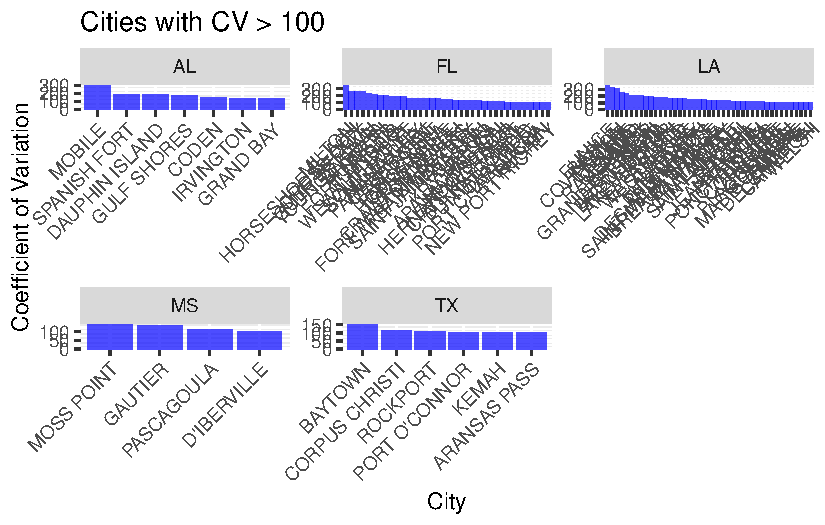
\includegraphics{CV_Communities2_files/figure-pdf/unnamed-chunk-9-1.pdf}

}

\end{figure}

Bar plot for FL and LA: High - Values

\begin{Shaded}
\begin{Highlighting}[]
\CommentTok{\# Filter FL and LA}
\NormalTok{fl\_la\_cities }\OtherTok{\textless{}{-}} \FunctionTok{subset}\NormalTok{(high\_cv\_cities, dealer\_state }\SpecialCharTok{\%in\%} \FunctionTok{c}\NormalTok{(}\StringTok{"FL"}\NormalTok{, }\StringTok{"LA"}\NormalTok{))}

\CommentTok{\# Bar plot for FL and LA}
\FunctionTok{ggplot}\NormalTok{(fl\_la\_cities, }\FunctionTok{aes}\NormalTok{(}\AttributeTok{x =} \FunctionTok{reorder}\NormalTok{(dealer\_city, }\SpecialCharTok{{-}}\NormalTok{Coefficient\_of\_Variation), }\AttributeTok{y =}\NormalTok{ Coefficient\_of\_Variation)) }\SpecialCharTok{+}
  \FunctionTok{geom\_bar}\NormalTok{(}\AttributeTok{stat =} \StringTok{"identity"}\NormalTok{, }\AttributeTok{fill =} \StringTok{"blue"}\NormalTok{, }\AttributeTok{alpha =} \FloatTok{0.7}\NormalTok{) }\SpecialCharTok{+}
  \FunctionTok{labs}\NormalTok{(}\AttributeTok{title =} \StringTok{"Cities with CV \textgreater{} 100 (FL and LA only)"}\NormalTok{, }\AttributeTok{x =} \StringTok{"City"}\NormalTok{, }\AttributeTok{y =} \StringTok{"Coefficient of Variation"}\NormalTok{) }\SpecialCharTok{+}
  \FunctionTok{theme}\NormalTok{(}\AttributeTok{axis.text.x =} \FunctionTok{element\_text}\NormalTok{(}\AttributeTok{angle =} \DecValTok{45}\NormalTok{, }\AttributeTok{hjust =} \DecValTok{1}\NormalTok{)) }\SpecialCharTok{+}
  \FunctionTok{facet\_wrap}\NormalTok{(}\SpecialCharTok{\textasciitilde{}}\NormalTok{ dealer\_state, }\AttributeTok{scales =} \StringTok{"free"}\NormalTok{)}
\end{Highlighting}
\end{Shaded}

\begin{figure}[H]

{\centering 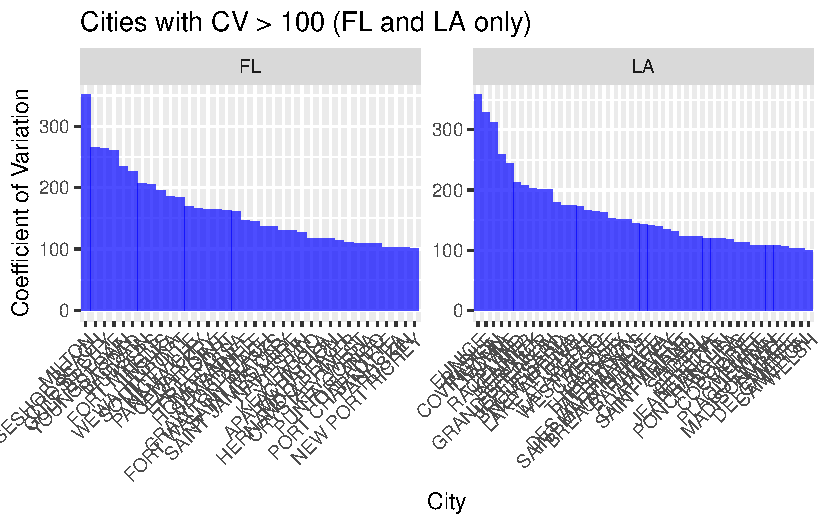
\includegraphics{CV_Communities2_files/figure-pdf/unnamed-chunk-10-1.pdf}

}

\end{figure}

Bar plot for Moderate Variability: High - Values

\begin{Shaded}
\begin{Highlighting}[]
\NormalTok{moderate\_CV\_val }\OtherTok{\textless{}{-}} \FunctionTok{subset}\NormalTok{(high\_variability\_cities, Coefficient\_of\_Variation }\SpecialCharTok{\textgreater{}} \DecValTok{30} \SpecialCharTok{\&}\NormalTok{ Coefficient\_of\_Variation }\SpecialCharTok{\textless{}=} \DecValTok{100}\NormalTok{)}

\CommentTok{\# Bar plot for cities with high CV, facet by state}
\FunctionTok{ggplot}\NormalTok{(moderate\_CV\_val, }\FunctionTok{aes}\NormalTok{(}\AttributeTok{x =} \FunctionTok{reorder}\NormalTok{(dealer\_city, }\SpecialCharTok{{-}}\NormalTok{Coefficient\_of\_Variation), }\AttributeTok{y =}\NormalTok{ Coefficient\_of\_Variation)) }\SpecialCharTok{+}
  \FunctionTok{geom\_bar}\NormalTok{(}\AttributeTok{stat =} \StringTok{"identity"}\NormalTok{, }\AttributeTok{fill =} \StringTok{"blue"}\NormalTok{, }\AttributeTok{alpha =} \FloatTok{0.7}\NormalTok{) }\SpecialCharTok{+}
  \FunctionTok{labs}\NormalTok{(}\AttributeTok{title =} \StringTok{"Cities with Moderate CV between 30\% and 100\%"}\NormalTok{, }\AttributeTok{x =} \StringTok{"City"}\NormalTok{, }\AttributeTok{y =} \StringTok{"Coefficient of Variation"}\NormalTok{) }\SpecialCharTok{+}
  \FunctionTok{theme}\NormalTok{(}\AttributeTok{axis.text.x =} \FunctionTok{element\_text}\NormalTok{(}\AttributeTok{angle =} \DecValTok{45}\NormalTok{, }\AttributeTok{hjust =} \DecValTok{1}\NormalTok{)) }\SpecialCharTok{+}
  \FunctionTok{facet\_wrap}\NormalTok{(}\SpecialCharTok{\textasciitilde{}}\NormalTok{ dealer\_state, }\AttributeTok{scales =} \StringTok{"free"}\NormalTok{)}
\end{Highlighting}
\end{Shaded}

\begin{figure}[H]

{\centering 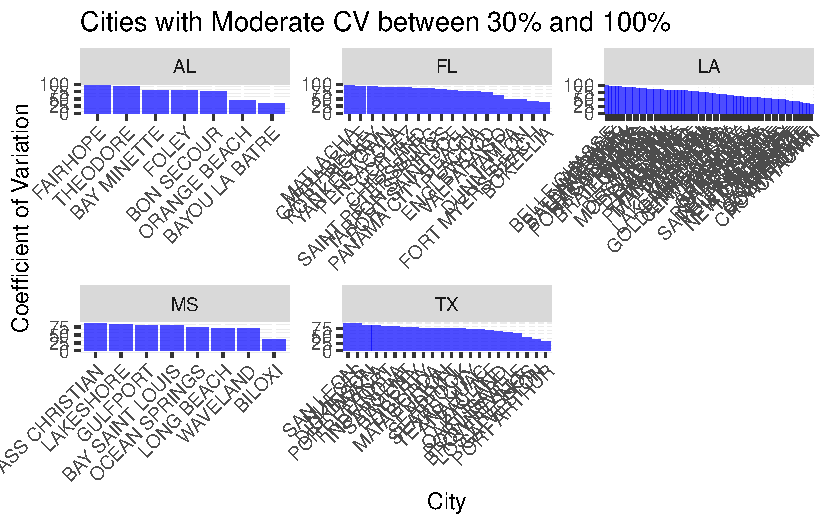
\includegraphics{CV_Communities2_files/figure-pdf/unnamed-chunk-11-1.pdf}

}

\end{figure}

Bar plot for FL and LA: moderate variability

\begin{Shaded}
\begin{Highlighting}[]
\CommentTok{\# Filter FL and LA}
\NormalTok{fl\_la\_cities\_M }\OtherTok{\textless{}{-}} \FunctionTok{subset}\NormalTok{(moderate\_CV\_val, dealer\_state }\SpecialCharTok{\%in\%} \FunctionTok{c}\NormalTok{(}\StringTok{"FL"}\NormalTok{, }\StringTok{"LA"}\NormalTok{))}
\CommentTok{\# Bar plot for FL and LA}
\FunctionTok{ggplot}\NormalTok{(fl\_la\_cities\_M, }\FunctionTok{aes}\NormalTok{(}\AttributeTok{x =} \FunctionTok{reorder}\NormalTok{(dealer\_city, }\SpecialCharTok{{-}}\NormalTok{Coefficient\_of\_Variation), }\AttributeTok{y =}\NormalTok{ Coefficient\_of\_Variation)) }\SpecialCharTok{+}
  \FunctionTok{geom\_bar}\NormalTok{(}\AttributeTok{stat =} \StringTok{"identity"}\NormalTok{, }\AttributeTok{fill =} \StringTok{"blue"}\NormalTok{, }\AttributeTok{alpha =} \FloatTok{0.7}\NormalTok{) }\SpecialCharTok{+}
  \FunctionTok{labs}\NormalTok{(}\AttributeTok{title =} \StringTok{"Cities with  Moderate CV between 30\% and 100\%"}\NormalTok{, }\AttributeTok{x =} \StringTok{"City"}\NormalTok{, }\AttributeTok{y =} \StringTok{"Coefficient of Variation"}\NormalTok{) }\SpecialCharTok{+}
  \FunctionTok{theme}\NormalTok{(}\AttributeTok{axis.text.x =} \FunctionTok{element\_text}\NormalTok{(}\AttributeTok{angle =} \DecValTok{45}\NormalTok{, }\AttributeTok{hjust =} \DecValTok{1}\NormalTok{)) }\SpecialCharTok{+}
  \FunctionTok{facet\_wrap}\NormalTok{(}\SpecialCharTok{\textasciitilde{}}\NormalTok{ dealer\_state, }\AttributeTok{scales =} \StringTok{"free"}\NormalTok{)}
\end{Highlighting}
\end{Shaded}

\begin{figure}[H]

{\centering 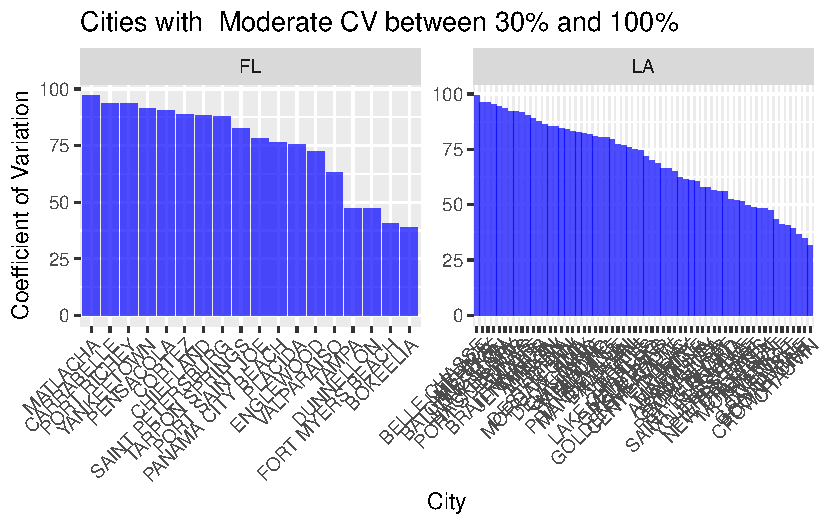
\includegraphics{CV_Communities2_files/figure-pdf/unnamed-chunk-12-1.pdf}

}

\end{figure}

\#\#2.Pounds:Calculate Coeficient of Variation for Total Landed Pounds

\begin{Shaded}
\begin{Highlighting}[]
\NormalTok{top\_10\_lbs }\OtherTok{\textless{}{-}}\NormalTok{ GI }\SpecialCharTok{\%\textgreater{}\%}
  \FunctionTok{filter}\NormalTok{(common\_name }\SpecialCharTok{\%in\%}\NormalTok{ Most\_Val) }\CommentTok{\# this has over 50,000 records which is much smaller than the original data file which has so many more species}
\end{Highlighting}
\end{Shaded}

Group by Year and City 2

This will give you the cumulative inflation-adjusted values for each
city in each year. Select only needed columns to avoid multiplication

\begin{Shaded}
\begin{Highlighting}[]
\FunctionTok{library}\NormalTok{(dplyr)}

\CommentTok{\# Step 1: Filter out rows with NA in dealer\_city}
\NormalTok{top\_10\_lbs }\OtherTok{\textless{}{-}}\NormalTok{ top\_10\_lbs }\SpecialCharTok{\%\textgreater{}\%}
  \FunctionTok{filter}\NormalTok{(dealer\_city }\SpecialCharTok{!=} \StringTok{"\#N/A"}\NormalTok{, }\SpecialCharTok{!}\FunctionTok{is.na}\NormalTok{(dealer\_city))  }\CommentTok{\# Exclude rows with *N/A and NAs in dealer\_city}

\NormalTok{top\_10\_lbs }\OtherTok{\textless{}{-}}\NormalTok{ top\_10\_lbs }\SpecialCharTok{\%\textgreater{}\%}
  \FunctionTok{filter}\NormalTok{(dealer\_city }\SpecialCharTok{!=} \StringTok{"UNRESOLVED"} \SpecialCharTok{\&}\NormalTok{ dealer\_city }\SpecialCharTok{!=} \StringTok{"UNKNOWN"}\NormalTok{)}


\CommentTok{\# Step 2: Filter for values greater than 1 in Adjusted\_Val}
\NormalTok{top\_10\_lbs }\OtherTok{\textless{}{-}}\NormalTok{ top\_10\_lbs }\SpecialCharTok{\%\textgreater{}\%}
  \FunctionTok{filter}\NormalTok{(live\_lbs }\SpecialCharTok{\textgreater{}} \DecValTok{1} \SpecialCharTok{\&} \SpecialCharTok{!}\FunctionTok{is.na}\NormalTok{(live\_lbs))}

\CommentTok{\# Select specific columns from top\_10\_data}
\NormalTok{Select\_columns\_lbs }\OtherTok{\textless{}{-}} \FunctionTok{c}\NormalTok{(}\StringTok{"landed\_year"}\NormalTok{, }\StringTok{"dealer\_city"}\NormalTok{, }\StringTok{"dealer\_state"}\NormalTok{, }\StringTok{"live\_lbs"}\NormalTok{)}
\NormalTok{select\_top\_lbs }\OtherTok{\textless{}{-}}\NormalTok{ top\_10\_lbs }\SpecialCharTok{\%\textgreater{}\%}
  \FunctionTok{select}\NormalTok{(}\FunctionTok{all\_of}\NormalTok{(Select\_columns\_lbs))}
\end{Highlighting}
\end{Shaded}

Group by landed year and city and calculate total values 2

\begin{Shaded}
\begin{Highlighting}[]
\CommentTok{\# Group by "landed\_year" and "dealer\_city" and include state information}
\NormalTok{grouped\_lbs }\OtherTok{\textless{}{-}}\NormalTok{select\_top\_lbs }\SpecialCharTok{\%\textgreater{}\%}
  \FunctionTok{group\_by}\NormalTok{(landed\_year, dealer\_city, dealer\_state) }\SpecialCharTok{\%\textgreater{}\%} \CommentTok{\#total for each year for city}
  \FunctionTok{summarize}\NormalTok{(}\AttributeTok{Total\_lbs =} \FunctionTok{sum}\NormalTok{(live\_lbs))}
\end{Highlighting}
\end{Shaded}

\begin{verbatim}
`summarise()` has grouped output by 'landed_year', 'dealer_city'. You can
override using the `.groups` argument.
\end{verbatim}

\begin{Shaded}
\begin{Highlighting}[]
\FunctionTok{head}\NormalTok{(grouped\_lbs)}
\end{Highlighting}
\end{Shaded}

\begin{verbatim}
# A tibble: 6 x 4
# Groups:   landed_year, dealer_city [6]
  landed_year dealer_city  dealer_state Total_lbs
        <int> <chr>        <chr>            <dbl>
1        1977 ABBEVILLE    LA              249225
2        1977 ANAHUAC      TX              749084
3        1977 APALACHICOLA FL             1283087
4        1977 ARANSAS PASS TX            19771196
5        1977 BARATARIA    LA             2373232
6        1977 BATON ROUGE  LA              865614
\end{verbatim}

Calculate Coefficient of Variation for Total Landed Pounds

\begin{Shaded}
\begin{Highlighting}[]
\NormalTok{cv\_lbs }\OtherTok{\textless{}{-}}\NormalTok{ grouped\_lbs }\SpecialCharTok{\%\textgreater{}\%}
  \FunctionTok{group\_by}\NormalTok{(dealer\_city, dealer\_state) }\SpecialCharTok{\%\textgreater{}\%}
  \FunctionTok{filter}\NormalTok{(}\FunctionTok{n}\NormalTok{() }\SpecialCharTok{\textgreater{}=} \DecValTok{10}\NormalTok{) }\SpecialCharTok{\%\textgreater{}\%}  \CommentTok{\# Keep groups with 10 or more data points for years}
  \FunctionTok{summarize}\NormalTok{(}
    \AttributeTok{Mean\_Total\_lbs =} \FunctionTok{mean}\NormalTok{(Total\_lbs, }\AttributeTok{na.rm =} \ConstantTok{TRUE}\NormalTok{),}
    \AttributeTok{SD\_Total\_lbs =} \FunctionTok{sd}\NormalTok{(Total\_lbs, }\AttributeTok{na.rm =} \ConstantTok{TRUE}\NormalTok{),}
    \AttributeTok{Coefficient\_of\_Variation =} \FunctionTok{ifelse}\NormalTok{(}\SpecialCharTok{!}\FunctionTok{is.na}\NormalTok{(SD\_Total\_lbs), }\FunctionTok{round}\NormalTok{((SD\_Total\_lbs }\SpecialCharTok{/}\NormalTok{ Mean\_Total\_lbs) }\SpecialCharTok{*} \DecValTok{100}\NormalTok{, }\DecValTok{2}\NormalTok{), }\ConstantTok{NA}\NormalTok{)}
\NormalTok{  )}
\end{Highlighting}
\end{Shaded}

\begin{verbatim}
`summarise()` has grouped output by 'dealer_city'. You can override using the
`.groups` argument.
\end{verbatim}

\#\#Identify Cities with High Variability: Pounds

\begin{Shaded}
\begin{Highlighting}[]
\NormalTok{high\_cities\_LBS }\OtherTok{\textless{}{-}}\NormalTok{ cv\_lbs[}\FunctionTok{order}\NormalTok{(}\SpecialCharTok{{-}}\NormalTok{cv\_lbs}\SpecialCharTok{$}\NormalTok{Coefficient\_of\_Variation), ]}

\FunctionTok{library}\NormalTok{(openxlsx)}

\CommentTok{\# Specify the full file path and name}
\NormalTok{file\_path }\OtherTok{\textless{}{-}} \StringTok{"C:/Users/Suzana.Mic/Documents/Resilience/CV\_Analysis/Output/high\_cities\_LBS.xlsx"}

\CommentTok{\# Write the DataFrame to an Excel file}
\FunctionTok{write.xlsx}\NormalTok{(high\_cities\_LBS, file\_path, }\AttributeTok{rowNames =} \ConstantTok{FALSE}\NormalTok{)}
\end{Highlighting}
\end{Shaded}

\#\#Graphical Representation Bar Plot High variability for Pounds Landed

\begin{Shaded}
\begin{Highlighting}[]
\FunctionTok{library}\NormalTok{(ggplot2)}

\CommentTok{\# Filter cities with CV \textgreater{} 100}
\NormalTok{cv\_cities\_lbs }\OtherTok{\textless{}{-}} \FunctionTok{subset}\NormalTok{(high\_cities\_LBS, Coefficient\_of\_Variation }\SpecialCharTok{\textgreater{}} \DecValTok{100}\NormalTok{)}


\CommentTok{\# Bar plot for cities with high CV, facet by state}
\FunctionTok{ggplot}\NormalTok{(cv\_cities\_lbs, }\FunctionTok{aes}\NormalTok{(}\AttributeTok{x =} \FunctionTok{reorder}\NormalTok{(dealer\_city, }\SpecialCharTok{{-}}\NormalTok{Coefficient\_of\_Variation), }\AttributeTok{y =}\NormalTok{ Coefficient\_of\_Variation)) }\SpecialCharTok{+}
  \FunctionTok{geom\_bar}\NormalTok{(}\AttributeTok{stat =} \StringTok{"identity"}\NormalTok{, }\AttributeTok{fill =} \StringTok{"blue"}\NormalTok{, }\AttributeTok{alpha =} \FloatTok{0.7}\NormalTok{) }\SpecialCharTok{+}
  \FunctionTok{labs}\NormalTok{(}\AttributeTok{title =} \StringTok{"Cities with CV \textgreater{} 100"}\NormalTok{, }\AttributeTok{x =} \StringTok{"City"}\NormalTok{, }\AttributeTok{y =} \StringTok{"Coefficient of Variation for Landed Pounds"}\NormalTok{) }\SpecialCharTok{+}
  \FunctionTok{theme}\NormalTok{(}\AttributeTok{axis.text.x =} \FunctionTok{element\_text}\NormalTok{(}\AttributeTok{angle =} \DecValTok{45}\NormalTok{, }\AttributeTok{hjust =} \DecValTok{1}\NormalTok{)) }\SpecialCharTok{+}
  \FunctionTok{facet\_wrap}\NormalTok{(}\SpecialCharTok{\textasciitilde{}}\NormalTok{ dealer\_state, }\AttributeTok{scales =} \StringTok{"free"}\NormalTok{)}
\end{Highlighting}
\end{Shaded}

\begin{figure}[H]

{\centering 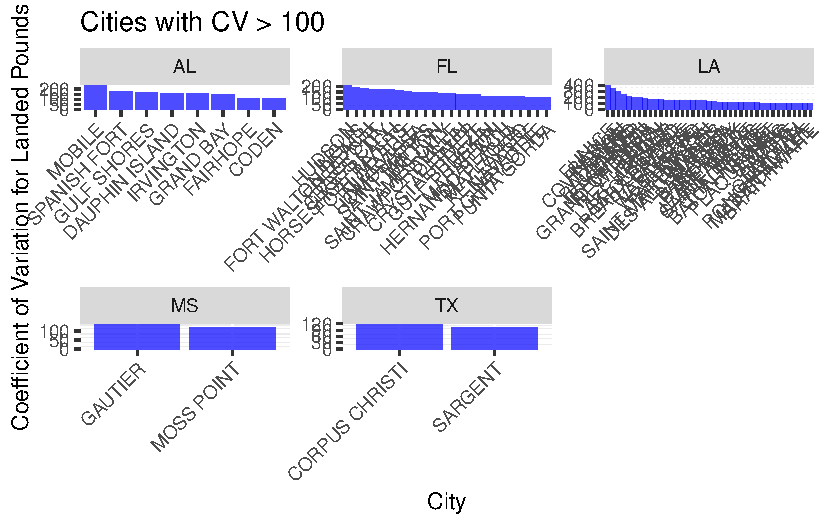
\includegraphics{CV_Communities2_files/figure-pdf/unnamed-chunk-18-1.pdf}

}

\end{figure}

Bar plot for FL and LA: High Variability Pounds Landed

\begin{Shaded}
\begin{Highlighting}[]
\CommentTok{\# Filter FL and LA}
\NormalTok{fl\_la\_cities\_lbs }\OtherTok{\textless{}{-}} \FunctionTok{subset}\NormalTok{(cv\_cities\_lbs, dealer\_state }\SpecialCharTok{\%in\%} \FunctionTok{c}\NormalTok{(}\StringTok{"FL"}\NormalTok{, }\StringTok{"LA"}\NormalTok{))}

\CommentTok{\# Bar plot for FL and LA}
\FunctionTok{ggplot}\NormalTok{(fl\_la\_cities\_lbs, }\FunctionTok{aes}\NormalTok{(}\AttributeTok{x =} \FunctionTok{reorder}\NormalTok{(dealer\_city, }\SpecialCharTok{{-}}\NormalTok{Coefficient\_of\_Variation), }\AttributeTok{y =}\NormalTok{ Coefficient\_of\_Variation)) }\SpecialCharTok{+}
  \FunctionTok{geom\_bar}\NormalTok{(}\AttributeTok{stat =} \StringTok{"identity"}\NormalTok{, }\AttributeTok{fill =} \StringTok{"blue"}\NormalTok{, }\AttributeTok{alpha =} \FloatTok{0.7}\NormalTok{) }\SpecialCharTok{+}
  \FunctionTok{labs}\NormalTok{(}\AttributeTok{title =} \StringTok{"Cities with CV \textgreater{} 100 (FL and LA only)"}\NormalTok{, }\AttributeTok{x =} \StringTok{"City"}\NormalTok{, }\AttributeTok{y =} \StringTok{"Coefficient of Variation for Landed Pounds"}\NormalTok{) }\SpecialCharTok{+}
  \FunctionTok{theme}\NormalTok{(}\AttributeTok{axis.text.x =} \FunctionTok{element\_text}\NormalTok{(}\AttributeTok{angle =} \DecValTok{45}\NormalTok{, }\AttributeTok{hjust =} \DecValTok{1}\NormalTok{)) }\SpecialCharTok{+}
  \FunctionTok{facet\_wrap}\NormalTok{(}\SpecialCharTok{\textasciitilde{}}\NormalTok{ dealer\_state, }\AttributeTok{scales =} \StringTok{"free"}\NormalTok{)}
\end{Highlighting}
\end{Shaded}

\begin{figure}[H]

{\centering 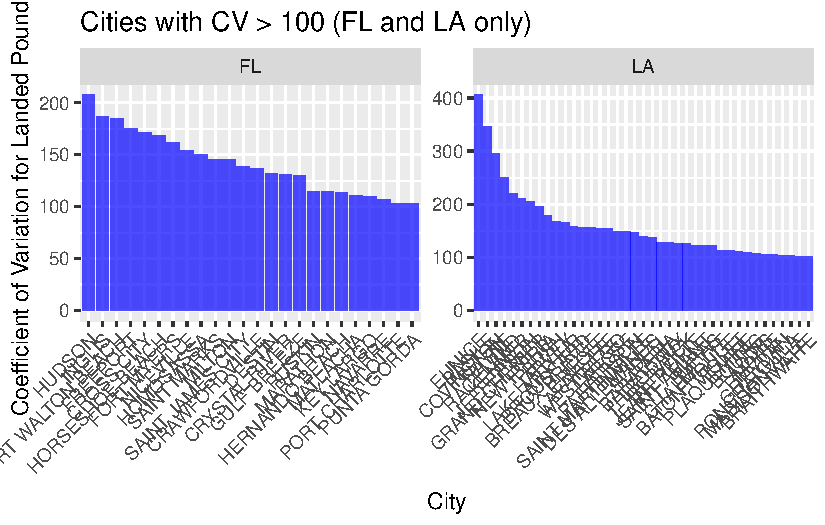
\includegraphics{CV_Communities2_files/figure-pdf/unnamed-chunk-19-1.pdf}

}

\end{figure}

\hypertarget{b.-identify-cities-with-low-variability}{%
\section{B. Identify Cities with Low
Variability}\label{b.-identify-cities-with-low-variability}}

\#\#1.Value of Landed Fish

\begin{Shaded}
\begin{Highlighting}[]
\CommentTok{\# Sort the DataFrame in descending order based on Coefficient\_of\_Variation}
\NormalTok{sorted\_low\_variability\_cities }\OtherTok{\textless{}{-}}\NormalTok{ cv\_data[}\FunctionTok{order}\NormalTok{(cv\_data}\SpecialCharTok{$}\NormalTok{Coefficient\_of\_Variation, }\AttributeTok{decreasing =} \ConstantTok{TRUE}\NormalTok{), ]}

\CommentTok{\# Filter cities with CV equal or smaller than 60}
\NormalTok{low\_variability\_cities }\OtherTok{\textless{}{-}}\NormalTok{ sorted\_low\_variability\_cities[sorted\_low\_variability\_cities}\SpecialCharTok{$}\NormalTok{Coefficient\_of\_Variation }\SpecialCharTok{\textless{}=} \DecValTok{60}\NormalTok{, ]}

\CommentTok{\# Specify the full file path and name for the low variability cities}
\NormalTok{file\_path\_low\_variability }\OtherTok{\textless{}{-}} \StringTok{"C:/Users/Suzana.Mic/Documents/Resilience/CV\_Analysis/Output/low\_variability\_cities.xlsx"}

\CommentTok{\# Write the DataFrame to an Excel file}
\FunctionTok{library}\NormalTok{(openxlsx)}
\FunctionTok{write.xlsx}\NormalTok{(low\_variability\_cities, file\_path\_low\_variability, }\AttributeTok{rowNames =} \ConstantTok{FALSE}\NormalTok{)}
\end{Highlighting}
\end{Shaded}

\#\#Graphical Representation: low variability Bar Plot

\begin{Shaded}
\begin{Highlighting}[]
\FunctionTok{library}\NormalTok{(ggplot2)}
\CommentTok{\# Filter cities with CV below 30\%}
\NormalTok{low\_variability\_cities }\OtherTok{\textless{}{-}} \FunctionTok{subset}\NormalTok{(low\_variability\_cities, Coefficient\_of\_Variation }\SpecialCharTok{\textless{}=} \DecValTok{30}\NormalTok{) }

\CommentTok{\# Bar plot for cities with low CV, facet by state}
\FunctionTok{ggplot}\NormalTok{(low\_variability\_cities, }\FunctionTok{aes}\NormalTok{(}\AttributeTok{x =} \FunctionTok{reorder}\NormalTok{(dealer\_city, Coefficient\_of\_Variation), }\AttributeTok{y =}\NormalTok{ Coefficient\_of\_Variation)) }\SpecialCharTok{+}
  \FunctionTok{geom\_bar}\NormalTok{(}\AttributeTok{stat =} \StringTok{"identity"}\NormalTok{, }\AttributeTok{fill =} \StringTok{"green"}\NormalTok{, }\AttributeTok{alpha =} \FloatTok{0.7}\NormalTok{) }\SpecialCharTok{+}
  \FunctionTok{labs}\NormalTok{(}\AttributeTok{title =} \StringTok{"Cities with Low Variability or a CV \textless{}= 30"}\NormalTok{, }\AttributeTok{x =} \StringTok{"City"}\NormalTok{, }\AttributeTok{y =} \StringTok{"Coefficient of Variation"}\NormalTok{) }\SpecialCharTok{+}
  \FunctionTok{theme}\NormalTok{(}\AttributeTok{axis.text.x =} \FunctionTok{element\_text}\NormalTok{(}\AttributeTok{angle =} \DecValTok{45}\NormalTok{, }\AttributeTok{hjust =} \DecValTok{1}\NormalTok{)) }\SpecialCharTok{+}
  \FunctionTok{facet\_wrap}\NormalTok{(}\SpecialCharTok{\textasciitilde{}}\NormalTok{ dealer\_state, }\AttributeTok{scales =} \StringTok{"free"}\NormalTok{)}
\end{Highlighting}
\end{Shaded}

\begin{figure}[H]

{\centering 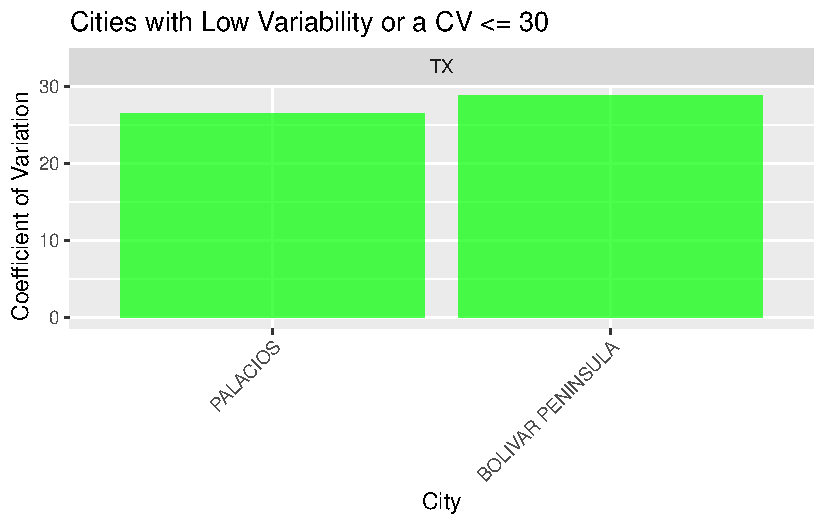
\includegraphics{CV_Communities2_files/figure-pdf/unnamed-chunk-21-1.pdf}

}

\end{figure}

\#\#1.Pounds of Landed Fish: Low variability

\begin{Shaded}
\begin{Highlighting}[]
\CommentTok{\#Sort the DataFrame in descending order based on Coefficient\_of\_Variation}
\NormalTok{sorted\_low\_variability\_cities\_LBS }\OtherTok{\textless{}{-}}\NormalTok{ cv\_lbs[}\FunctionTok{order}\NormalTok{(cv\_lbs}\SpecialCharTok{$}\NormalTok{Coefficient\_of\_Variation, }\AttributeTok{decreasing =} \ConstantTok{TRUE}\NormalTok{), ]}

\CommentTok{\# Filter cities with CV equal or smaller than 60}
\NormalTok{low\_variability\_cities\_LBS }\OtherTok{\textless{}{-}}\NormalTok{ sorted\_low\_variability\_cities\_LBS[sorted\_low\_variability\_cities\_LBS}\SpecialCharTok{$}\NormalTok{Coefficient\_of\_Variation }\SpecialCharTok{\textless{}=} \DecValTok{30}\NormalTok{, ]}

\FunctionTok{library}\NormalTok{(openxlsx)}

\CommentTok{\# Specify the full file path and name}
\NormalTok{file\_path }\OtherTok{\textless{}{-}} \StringTok{"C:/Users/Suzana.Mic/Documents/Resilience/CV\_Analysis/Output/low\_variability\_cities\_LBS.xlsx"}

\CommentTok{\# Write the DataFrame to an Excel file}
\FunctionTok{write.xlsx}\NormalTok{(low\_variability\_cities\_LBS, file\_path, }\AttributeTok{rowNames =} \ConstantTok{FALSE}\NormalTok{)}
\end{Highlighting}
\end{Shaded}

\#\#Graphical Representation Bar Plot

\begin{Shaded}
\begin{Highlighting}[]
\FunctionTok{library}\NormalTok{(ggplot2)}

\CommentTok{\# Bar plot for cities with high CV, facet by state}
\FunctionTok{ggplot}\NormalTok{(low\_variability\_cities\_LBS, }\FunctionTok{aes}\NormalTok{(}\AttributeTok{x =} \FunctionTok{reorder}\NormalTok{(dealer\_city, }\SpecialCharTok{{-}}\NormalTok{Coefficient\_of\_Variation), }\AttributeTok{y =}\NormalTok{ Coefficient\_of\_Variation)) }\SpecialCharTok{+}
  \FunctionTok{geom\_bar}\NormalTok{(}\AttributeTok{stat =} \StringTok{"identity"}\NormalTok{, }\AttributeTok{fill =} \StringTok{"blue"}\NormalTok{, }\AttributeTok{alpha =} \FloatTok{0.7}\NormalTok{) }\SpecialCharTok{+}
  \FunctionTok{labs}\NormalTok{(}\AttributeTok{title =} \StringTok{"Cities with Low relative Variability or CV \textless{}= 30"}\NormalTok{, }\AttributeTok{x =} \StringTok{"City"}\NormalTok{, }\AttributeTok{y =} \StringTok{"Coefficient of Variation for Landed Pounds"}\NormalTok{) }\SpecialCharTok{+}
  \FunctionTok{theme}\NormalTok{(}\AttributeTok{axis.text.x =} \FunctionTok{element\_text}\NormalTok{(}\AttributeTok{angle =} \DecValTok{45}\NormalTok{, }\AttributeTok{hjust =} \DecValTok{1}\NormalTok{)) }\SpecialCharTok{+}
  \FunctionTok{facet\_wrap}\NormalTok{(}\SpecialCharTok{\textasciitilde{}}\NormalTok{ dealer\_state, }\AttributeTok{scales =} \StringTok{"free"}\NormalTok{)}
\end{Highlighting}
\end{Shaded}

\begin{figure}[H]

{\centering 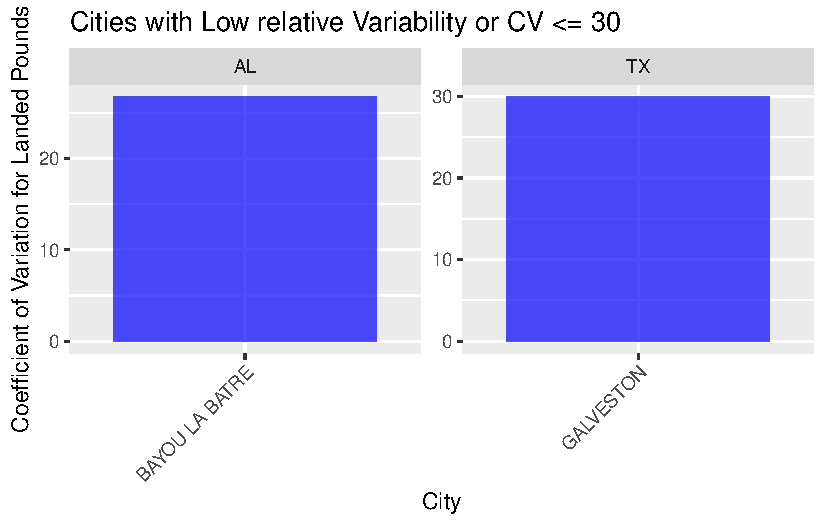
\includegraphics{CV_Communities2_files/figure-pdf/unnamed-chunk-23-1.pdf}

}

\end{figure}



\end{document}
